\documentclass[11p, titlepage]{article}

\usepackage[a4paper, portrait, margin=0.9in]{geometry}
\setlength{\parskip}{1em}

\usepackage[hidelinks]{hyperref}

\usepackage{graphicx}
\graphicspath{ {./images/} }
\usepackage{caption}
\usepackage{subcaption}
\captionsetup[subfigure]{justification=centering}
\usepackage{wrapfig}

\title{COSC470 Research Project Report\\
\bigskip
Contour Splitting for Branching Structures in CT Image Reconstructions}
\author{Cameron Stevenson\\[0.5cm]{\small Supervisor: Ramakrishnan Mukundan}}

\begin{document}

\maketitle
\abstract{abstract text}
\tableofcontents

\section{Overview}

overview text
Example citation \cite{mackay2019robust, mukundan2016reconstruction, pan2017comparison}.
Example URL \footnote{\url{https://github.com/cstevenson3/cosc470writing/blob/main/survey.pdf}}.

\section{Introduction}

introduction text

\section{Background}

We begin with a look at typical methods in rendering scan data. Then, correspondence methods are looked at in depth as the approach this report builds upon.

\subsection{Overview}

Images from scans (also referred to as sections or slices) can be segmented based on intensity into pixel regions to define structure boundaries. These can be processed further by finding contours to represent these boundaries.

Any medical imaging reconstruction/render is typically concerned with a particular area of the body, dependent on the application. Most applications tend to use either volumetric rendering or surface rendering.

Volumetric rendering treats pixels in images as voxels, and a variety of rasterization and raycasting techniques are available for rendering these.

Surface rendering requires a surface be defined, either implicitly or as a mesh. Point cloud methods generate implicit surfaces, whilst meshes can be generated through contour correspondence followed by mesh triangulation (with point correspondence as an optional middle step). 

\subsection{Applications}

Xuyi et al. \cite{xuyi2016application} use 3D reconstructions from hip CT scans to make patient-specific surgery plans. From the model they measure the direction and degree of the acetabular fragment, and use this to guide their surgery.

Pan et al. \cite{pan2017comparison} refers to the importance of 3D reconstructions and rendering in robot-assisted surgery. With real time rendering being a priority, surface reconstructions are preferred over volume rendering. Of the four methods analysed, marching cubes was found to be the most suitable due to its speed and render quality.

Lim et al \cite{lim2016use} found that the use of 3D printed cardiac models in education resulted in a statistically significant improvement in test scores of medical students.

\subsection{Scanning and Image Processing}

As with most areas involving measurement of the real world, unwanted artefacts such as noise are introduced in the imaging process. There can also be variation from subject to subject and between imaging machines. Therefore standard image processing techniques are used to pick out the parts of images which are relevant to the application. Running signal processing on the 2D data (as opposed to considering the whole image stack in the reconstruction stage) reduces complexity. However techniques considering the image data from all slices have been considered.

\subsubsection{Segmentation}

Segmentation is the process of picking out the pixels belonging to individual objects in an image. From this the projected geometry of the object onto the image can be inferred, which is then used in reconstruction or rendering. Birkfellner \cite{birkfellner2016applied} observes that organs are usually composed of multiple tissue types, which show up as different intensities under imaging. This makes segmentation "a rather complex, specialized procedure often requiring considerable manual interaction". Particular organs are often focussed on when developing segmentation methods.

Birkfellner \cite{birkfellner2016applied} covers some advanced segmentation methods. The watershed transform for example uses the physical idea of water running to the bottom of valleys in a landscape. After taking a gradient transform on an image, edges are peaks in the landscape, and the virtual water will fill up basins representing segments in the image. Various interpretations of the physical behaviour can be used.

Carr \cite{carr1996surface} refers to various morphological methods used to remove noise. An opening operation acts like a low pass filter whilst still preserving edges. Opening and closing in sequence tends to be better at maintaining the mean intensity.

Mukundan \cite{mukundan2016reconstruction} observes that in HRCT lung scans, tissue regions are "characterized by different and easily separable intensity levels". In this case simple thresholding can be used to pick out regions. 

\subsubsection{Contour Finding}

Rather than use pixels/voxels, some reconstruction techniques use contours defining the boundaries of the region objects occupy in an image. 

Mukundan \cite{mukundan2016reconstruction} starts with a binary image after thresholding. Eroding the image with a 3x3 element then subtracting this from the thresholded image gives one pixel wide edges. Sequential edge following is used to extract contours. Discarding small contours reduces the number of contours significantly.

Pu et al. \cite{pu2008adaptive} introduce a border marching algorithm with an adaptive step size to find the outer contours of the lungs. The metric for adjusting the step size for a border segment is based on how far (at most) the segment lies from the true border. This method has the advantage of including small juxtapleural pulmonary modules in the segmentation despite their imaged intensity being dissimilar to the rest of the lung. Mackay \cite{mackay2019robust} uses this method.

\subsubsection{Contour Interpolation}

Between two slices filled with contours, new slices can be added with contours interpolated from those in the slices above and below them. Some methods are able to do this without a contour correspondence.

Barrett et al. \cite{barrett1994image} present a contour interpolation algorithm in image space based on morphological operations. An image with both contours present (as different grayscale values) is dilated until the space between contours is filled. The front where the two dilations meet is where the interpolated contour is found. It is noted that this method handles branching cases with no modification necessary.

Chai et al. \cite{chai1998contour} use partial differential equations to interpolate between contours on a terrain map. Their method produces smooth interpolations, and can handle complex shapes such as two or three branches.

\subsection{Typical Methods}

generic methods text

\subsubsection{Volumetric Rendering}

Each image in the image stack is treated as a slice with thickness. Thus the pixels in the image are voxels, and various volume rendering techniques can be used to directly render the data without an intermediate structural representation such as a mesh. Since every voxel may be involved in the final render, naive implementations can be expensive. Techniques to improve the render quality and performance have been investigated.

\paragraph{Rasterization}

In rasterization, the forward direction of an object's effect on an image is considered. Each voxel may directly affect the final render, or first be projected onto a intermediate object which is then itself drawn.

Splatting takes each voxel's value and "splats" it against the drawn image, contributing to a few pixels, with its contribution fading away as you move outwards. Zwicker et al. \cite{zwicker2002ewa} use elliptic Gaussian kernels as the basis of the shape of each splat.

Texture-based volume rendering intersects many planes with the volume \cite{ohiotexture}. On these planes polygons are rendered, with texture mappings from their coordinates to the 3D space of the volume, to pull texture values from the voxels. The planes must not be parallel to the viewing direction.

\paragraph{Raycasting}

In raycasting, we take each pixel of the render and work backwards to find which objects affect it. Each pixel emits a ray which intersects with many voxels. The weighting of voxels is dependent on the technique.

Maximum intensity projection (MIP) is a raycasting method where rays project the most intense voxel they pass through \cite{birkfellner2016applied}. The images produced have high contrast detail and are easy to understand. Summed voxel rendering is another raycasting method where rays sum up intensities from every voxel they pass through, giving a blurred image \cite{birkfellner2016applied}.

Fishman et al. \cite{fishman2006volume} make comparisons between maximum intensity projection and other volume rendering. MIP tends to not contrast the background well with the structure of interest. Other volume rendering methods can weight voxels differently and give different tissue types different colours. 

Intersecting arbitrary rays with voxels can be computationally expensive. Shear-warp rendering solves this by using projections which make rays orthogonal to the voxel axes \cite{lacroute1994fast}. 

\subsubsection{Surface Reconstructions}

In each image of the image stack, we can see where the boundaries of tissue are. We can therefore describe the geometry of a structure as it intersects the image plane. By combining all images in the stack, a surface reconstruction of the entire object can be found, provided the relationships between slices are inferred accurately. Surfaces have the advantage of having commonplace rendering techniques, and support on 3D printers.

\paragraph{Marching Cubes}

Marching cubes \cite{lorensen1987marching} converts voxels into surfaces. Each voxel either belongs to a structure or does not, based on imaged intensity. Surface voxels ("inside" voxels bordering "outside" voxels, on some isosurface) are found. Each voxel has its corners defined as inside or outside based on its neighbours, and is then assigned a set of triangles based on those corners, using a lookup table. The triangles are joined in neighbouring surface voxels to form the overall mesh. The results tend to look jagged, and smoothing is usually applied either to the mesh or during rendering for a more visually accurate output.

Newman et al. \cite{newman2006survey} have conducted a comprehensive survey of marching cubes. One problem marching cubes has is ambiguity which induces defects. The survey recommends avoiding lookup tables with reflective symmetry, where "outside" and "inside" corners of a voxel are swapped to give the same triangle set but with opposite normals. Instead only rotational symmetry (rotating corners around the voxel) is allowed. Such a lookup table was identified by Nielson et al. \cite{nielson2003marching}.

\paragraph{Point Cloud Methods}

One of the more general ways of defining a surface with incomplete data is by sampling many points from it, and making assumptions about the way these points would be connected. This is common in 3D depth scanning of exteriors of objects, where many points are sampled but the entire surface is not known and must be inferred. If we treat the boundaries of tissue regions in images as sets of points, we can apply point cloud methods to all the points gathered. The techniques can be tuned for specific applications. Approximating methods produce surfaces which lean more heavily on the assumptions made, with the points guiding the end results. This is useful when the sampling of the points is noisy. Methods which interpolate assume the points are perfect and so the surfaces produced must pass through them. It is common to define a function from 3D space to a value so that the surface should be found where the function output is zero, then an isosurface at zero is generated.

\subparagraph{Models}

Braude et al. \cite{braude2007contour} employ Multi-level Partition of Unity (MPU) implicit models to generate isosurfaces from. MPU closely approximates Euclidean distance near points. This method requires surface normals. 

Guennebaud et al. \cite{guennebaud2007algebraic} fit algebraic spheres to point sets to construct surfaces. Their method (APSS) performs better than prior methods on sharp features and sparse data.

Oztireli et al. \cite{oztireli2009feature} combine Moving Least Squares (MLS) with local kernel regression to obtain Robust Implicit Moving Least Squares (RIMLS). This method reconstructs sharp (non-smooth) corners more accurately than APSS.

Taubin et al. \cite{taubin2012smooth} demonstrate colour maps extrapolated from source points onto a reconstructed surface.

\subparagraph{Estimating Normals}

Some of the methods above require normals for each point. Estimating normals from the points sampled requires some understanding of the structure itself.

Mitra et al. \cite{mitra2003estimating} use least squares distance to fit a plane to a neighbourhood of points for each point in the cloud. There is a sweet spot for the radius of the neighbourhood used. Small radius makes noisy points have more impact on the plane found, and large radius allows for surface curvature to introduce error. 

\paragraph{Mesh Rendering}

Mackay \cite{mackay2019robust} states that surface rendering is not as widely implemented as volume rendering in medical contexts. However mesh rendering is abundant in literature from applications such as video games. Should mesh reconstruction become more accurate and faster, more implementations of mesh rendering for medical imaging may become available.

\subsection{Testing}

The end aim of these reconstructions and renders is to give humans a better visualisation of internal structures. However to compare methods objective testing is required. Requiring human experts to come to a consensus on desired outputs is resource consuming for stages such as image segmentation, and infeasible for complex structures such as meshes. Therefore metrics and repeatable methods have been devised to test algorithms.

\subsubsection{Measuring Similarity in Segmentation}

Pixel-wise XOR operations are common, simply working out where an ideal segmentation and an output segmentation differ.

Pu et al. \cite{pu2008adaptive} use a reference segmentation contour (defined by experts), and evaluate the distribution of distance error along their result contour from this reference. 

\subsubsection{Generating Models}

It is difficult to obtain real models of internal structures. Techniques to generate synthetic models suitable for testing have been developed.

Mackay \cite{mackay2019robust} uses Blender3D to create test models, by creating surface of revolutions about bezier curves. Multiple surfaces are merged for more complex structures such as branches. The main intent here was to create simple models of problem structures. Contours can be sampled from these models by plane intersections.

Mackay \cite{mackay2019robust} also proposes an alternative method of generating test data, where a side view of a branching structure is drawn in black. An inter-slice distance is defined to separate rows. Each row is scanned for black pixels. When a black pixel is encountered, a contour is generated by revolving points about this pixel location. Noise can be added in. Where contours intersect, they are merged. This allows for branching structures to be generated by this method.

Pluta et al. \cite{pluta2012new} propose a rule-based method of generating lung models, including deformations and noise. Their rules are based on airflow and measured constants, and the distribution of final bronchioles in a lung. Their results are suitably accurate for testing all parts of lung reconstruction methods.

\subsubsection{Measuring Similarity in 3D Models}

Mackay \cite{mackay2019robust} uses Hausdorff distance (essentially a maximum deviation between point sets) to measure mesh similarity. Points are sampled from a ground truth model and the nearest distance is found to the reconstructed model.

Meshes can be sliced at the same heights and compared slicewise to reduce similarity to a 2D problem.

Shum et al. \cite{shum19963d} compare simple 3D objects by comparing the curvature of points based on spherical coordinates. This could be applied locally on more complex medical reconstructions.

\subsection{Performance}

Recent papers in medical imaging reconstructions tend to have an emphasis on taking advantage of modern hardware. This can be achieved through parallelization or GPU implementations.

Saxena et al. \cite{saxena2013image} describe parallel techniques for various image processing tasks such as segmentation and noise reduction. The main idea is to tile an image and let different processors work on different tiles, then deal with the borders when recombining the tiles. They found their parallel implementation to be 2.5 times faster than a sequential implementation.

Alsmirat et al. \cite{alsmirat2017accelerating} investigate pure GPU and hybrid CPU-GPU implementations of segmentation of medical images. They found that both outperform a CPU only implementation, and the hybrid method performs the best.

\subsection{Correspondence Methods}

correspondence methods text

\subsubsection{Contour Correspondence}

Rather than lose the relationship between points, the original contours can be used in creating a surface reconstruction. Working out which contours on which slices represent a connected tissue in the original structure is called contour correspondence, and the resulting correspondences are used in later steps of reconstruction.
\newline
\linebreak
Herbert et al. \cite{herbert2001contour} classify correspondence algorithms into four types. \begin{itemize}
\item Manual methods use user input to connect contours. This is time consuming for large datasets.
\item Local algorithms takes pairs of slices at a time and considers contour matchings between these.
\item Global algorithms look for contour pairings across all sections.
\item Growing algorithms create a hierarchy of components, attempting to join unmatched contours onto existing components if suitable.
\end{itemize}

Contour centroid position comparison is common in local algorithms.

Herbert et al. \cite{herbert2001contour} suggest growing objects one contour at a time instead of considering pairings of contours globally. In preprocessing spacial information is gathered such as contour characteristics (position, shape, size), intra-sectional relationships between contours (to validate complex structures later), and inter-sectional relationships. Contour relationship metrics include distance between centroids, distance between major/minor axes, minimum bounding rectangle overlap, shape comparison via compactness ratios, and surroundness (how deep is the contour nested in larger contours).

Herbert et al. \cite{herbert2001contour} include semantic information given by the user on the expected components in a reconstruction, and their spatial relation to each other. A starting contour is found for each component before the growing process starts.

Mukundan \cite{mukundan2016reconstruction} begins point correspondence without an explicit contour correspondence already found. If two point correspondences are found as neighbours belonging to the same pair of contours, the search for further point correspondences is narrowed to these two contours. This effectively gives a temporary contour correspondence.

\subsubsection{Point Correspondence}
Point correspondence is an optional step in surface reconstructions, where points on matched contours are matched to each other as a precursor to triangulation.

Mukundan \cite{mukundan2016reconstruction} uses distance in the XZ plane as a metric for matching points. Other optional constraints include matching the next point close to the previous point.

Mackay \cite{mackay2019robust} proposes Dynamic Time Warping (DTW) as a method of point correspondence. DTW is intended to match features on the same structure across different times. In point correspondence, it matches points on contours which are from the same structure but in different slices, so slightly warped. At any time during DTW a pair of points from both contours is matched, then the next points in both contours are considered as matches for the current points. DTW has some basic constraints when finding a warp path, but Mackay suggests adding further constraints as a potential improvement.

\subsubsection{Mesh Triangulation}

A surface can be represented as a set of primitive elements, with triangles being the simplest. They are defined by three points in 3D space. The final step of mesh reconstruction is taking the relationships inferred by contour and point correspondence, and generating triangles to connect points whilst taking these relationships into account.

Mackay \cite{mackay2019robust} begins with two ordered sets of points X and Y, from the two contours matched, with some edges provided by point correspondence. As a result of the constraints on DTW, there are three cases for each point $x_{m}$ on the first contour:
\begin{itemize}
\item $x_{m}$ has an edge with $y_{n}$ and $x_{m+1}$ has an edge with $y_{n+1}$. These points are direct neighbours on their respective contours, and form a quad which is trivial to triangulate.
\item $x_{m}$ has edges with a sequence of points $\{y_{n}, y_{n+1}, ..., y_{n+i}\}$. $x_{m}$ has a one-to-many point correspondence with these points. This can be triangulated with a triangle fan centering about $x_{m}$.
\item Each point in the sequence $\{x_{m}, x_{m+1}, ..., x_{m+i}\}$ has edges with a point $y_{n}$. This is the opposite of the previous case and can likewise be triangulated with a triangle fan centering about $y_{n}$.
\end{itemize}
Li et al. \cite{li2021method} observe that when m and n differ greatly, one-to-many point correspondences are common, and the triangulation becomes rough.

\subsubsection{Branching Problem}

A simple structure is easy to infer from its images. On each slice the structure is present in, we see one contour, and these contours are similarly positioned and shaped in adjacent slices. More complex structures such as a branch show up differently, and it becomes harder to infer the original structure. Contour correspondence must be adjusted to deduce these unusual structures when they appear. Even when the general layout of the original structure is inferred through contour correspondence, point correspondence and mesh triangulation can be difficult when the shapes of contours change suddenly.

Mackay \cite{mackay2019robust} looks for lung branches as one contour approximately splitting in half into two contours, for contour correspondence.

Mackay \cite{mackay2019robust} uses contour merging to help DTW point correspondence in the branching case. In a contour correspondence where there is a slice with a single contour and a slice with two contours, the two contours on the same slice are merged at their nearest point to give one larger contour. Point correspondence between the single contour and the merged contour can then proceed as normal. In some branching cases however, the triangulated mesh is twisted, as though DTW has not matched the correct points together. This problem is left for further research.

\subsection{Background Summary}

summary text

\section{Method}

method text

\subsection{Proposal}

\begin{wrapfigure}{r}{0.25\textwidth}
\centering
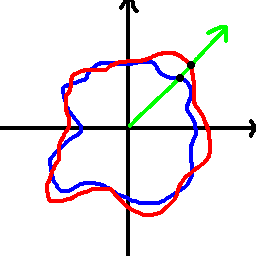
\includegraphics[width=0.2\textwidth]{pa}
\caption{Points matched by angle from shared centroid\label{fig:pa}}
\end{wrapfigure}

The proposed system consists of:
\begin{itemize}
\item Contour Splitting, a new approach to enabling point correspondence on branches and other structures
\item Point Angle, an alternative algorithm for point correspondence.
\end{itemize}

Example figure ref (See Figure \ref{fig:pa}).

\subsubsection{Contour Splitting}

For brevity, contour correspondences of 1-to-2 will be considered. Point correspondence algorithms act on 1-to-1 contour matchings, so 1-to-2 cases must be reduced to these. 

Mackay's approach was contour merging, where the 2 contour side of the correspondence is merged. The closest pair of points across the contours is found, to join them into a single contour (See Figure TODO). This gives a single 1-to-1 case for point correspondence to act on. A disadvantage of this method is that the merged contour has an unusual shape, which can cause point correspondence algorithms to behave poorly.

The proposed technique instead splits the 1 contour side of the correspondence. The best fit line to divide the 2 contour side is found, giving the angle of the line to split the 1 contour (See Figure TODO). Each half of the split 1 contour is paired with its corresponding contour on the 2 contour side. This gives two 1-to-1 cases for point correspondence to act on. The contours produced are well shaped and suitable for point correspondence algorithms designed for simpler cases.

Adjustments can be made to the position of the split line to improve accuracy. 
\begin{itemize}
\item The ratio of contour areas on the 2 contour side can be reflected in the split contour by adjusting which points the split line connects to. This preserves the internal cross section of each branch half as they join. 
\item To achieve a smooth point correspondence along the inside of the branch (where the branches join each other), the split line must have points added along it. This is in proportion to the number of points on the original contour.
\item The split line may also be adjusted in height, to reflect the likelihood the branch split is somewhere between the two planes of contours. With no further calculation, the height is assumed to be halfway. A semi-circular curve creates a split line joint which mimics the intersection of two cylinders, which is approximately what is expected from two branches coming together.
\end{itemize}

\subsubsection{Point Angle}

Prior methods of point correspondence consider the Euclidean distance between points on corresponded contours. The proposed algorithm instead considers similar angular distance relative to the contour's centroid. For contours where every border point can be seen from the centroid (similar to star-shaped polygons), the angular distance metric is monotonically increasing. In point correspondence, the contours' point angle metrics are leapfrogged between to join points (See Figure TODO). This leapfrogging assumes the monotonically increasing property. For contours which "double back" (are not star-shaped), the monotonically increasing property can be enforced when filling in the point angle metric, by recording the previous angle if the current angle is smaller. This can lead to sections of points with the same point angle metric, and leapfrogging which produces unideal many-to-one mappings. To counter this, a second metric is added, which is simply progression along the number of points in the contour, starting from the same point as the angle metric. These two metrics are weighted and summed before the leapfrogging correspondence.

\subsection{Implementation}

Mackay's report provides a complete implementation of contour and point correspondence (TODO cite software). This implementation was modified to add the options of contour splitting and point angle for point correspondence. The modified source code is available here (TODO git link).

\section{Analysis}

To analyse the effectiveness of the proposed method in improving reconstruction accuracy, synthetic models are intersected with planes to give contours of points, which are then given as input to reconstruction. These reconstructions from different methods are compared to the original and against each other. These observations are then confirmed with objective measurements such as Hausdorff distance.

\subsection{Ground Truth}

For ground truth we use the same synthetic models Mackay generated for analysis (See Figure \ref{fig:original_models}). Planes are intersected with the models to give the contours of points expected from scanning and segmenting a real object of the same shape. Plane counts of 10, 20, 30, 40 and 50 are used to emulate different scan slice thicknesses.

Additionally, Meshlab was used to copy specific sections of these models into new files, to focus reconstructions on the difficult cases the proposed method is intended to improve on. These are named after the original model and which slice range (based on the 10 slice levels version) is being copied.

\begin{figure}[h]
     \centering
     \begin{subfigure}[b]{0.3\textwidth}
         \centering
         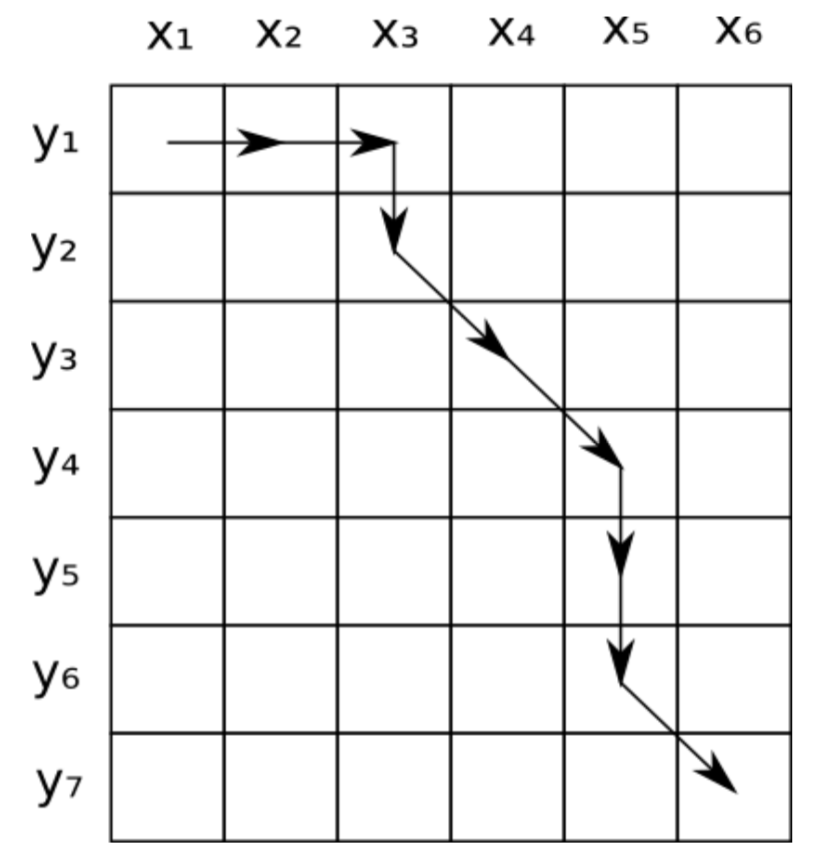
\includegraphics[width=\textwidth]{originals/simple}
         \caption{simple}
         \label{fig:simple}
     \end{subfigure}
     \hfill
     \begin{subfigure}[b]{0.3\textwidth}
         \centering
         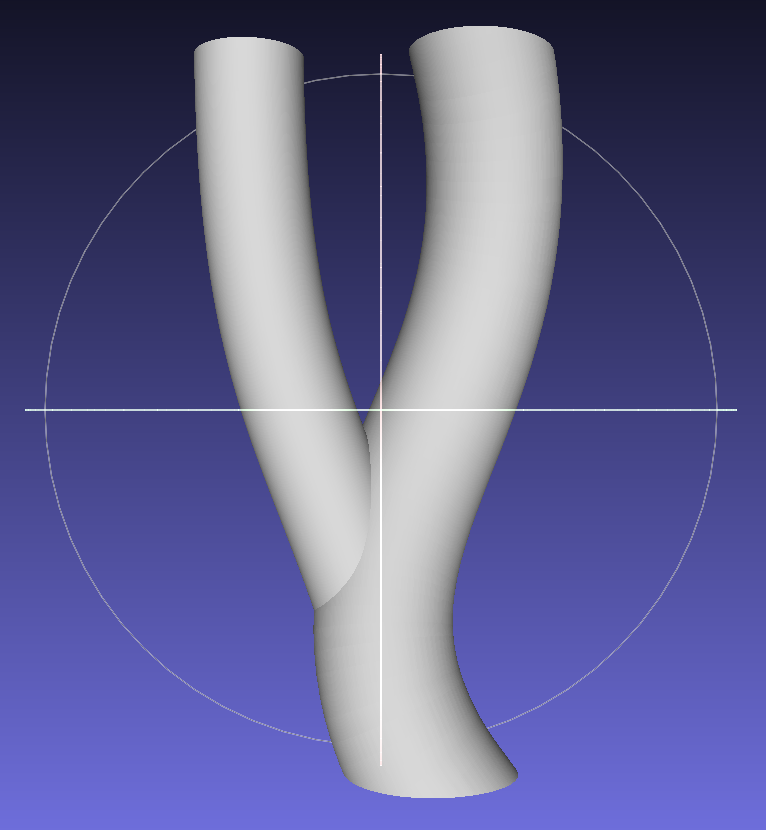
\includegraphics[width=\textwidth]{originals/simple-branch}
         \caption{simple-branch}
         \label{fig:simple_branch}
     \end{subfigure}
     \hfill
     \begin{subfigure}[b]{0.3\textwidth}
         \centering
         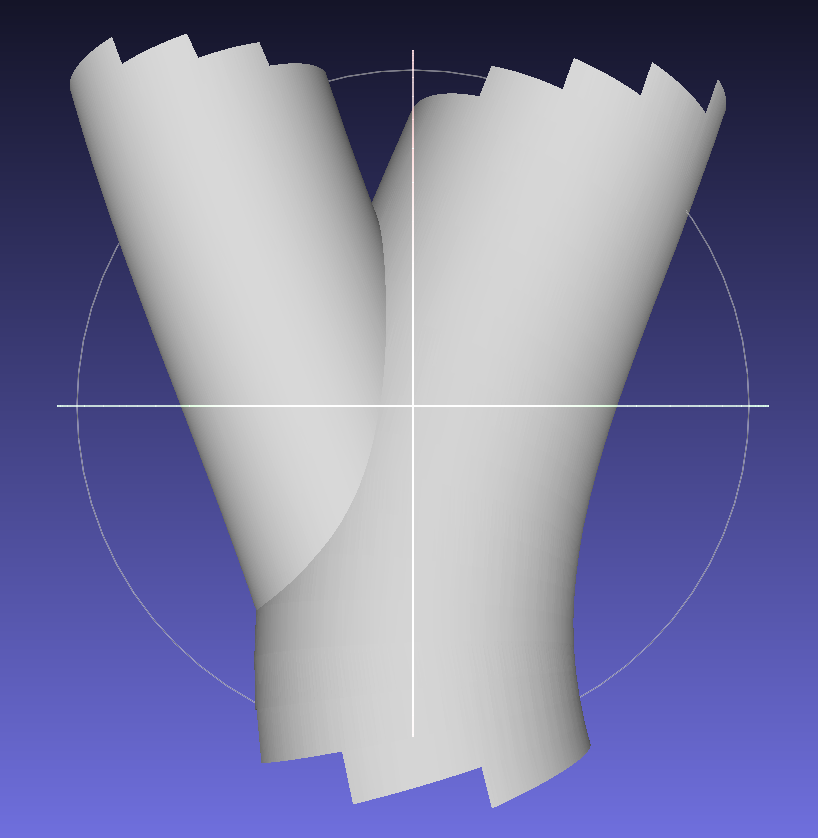
\includegraphics[width=\textwidth]{originals/simple-branch-2-6}
         \caption{simple-branch-2-6}
         \label{fig:simple_branch_focussed}
     \end{subfigure}
     \hfill
     \begin{subfigure}[b]{0.3\textwidth}
         \centering
         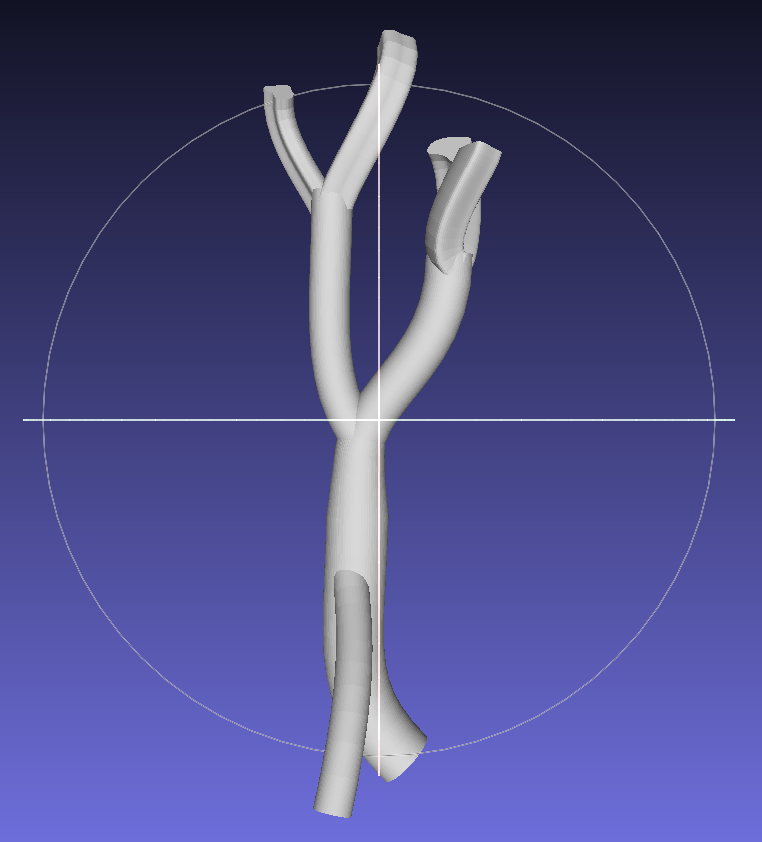
\includegraphics[width=\textwidth]{originals/multi-branch}
         \caption{multi-branch}
         \label{fig:multi_branch}
     \end{subfigure}
     \hfill
     \begin{subfigure}[b]{0.3\textwidth}
         \centering
         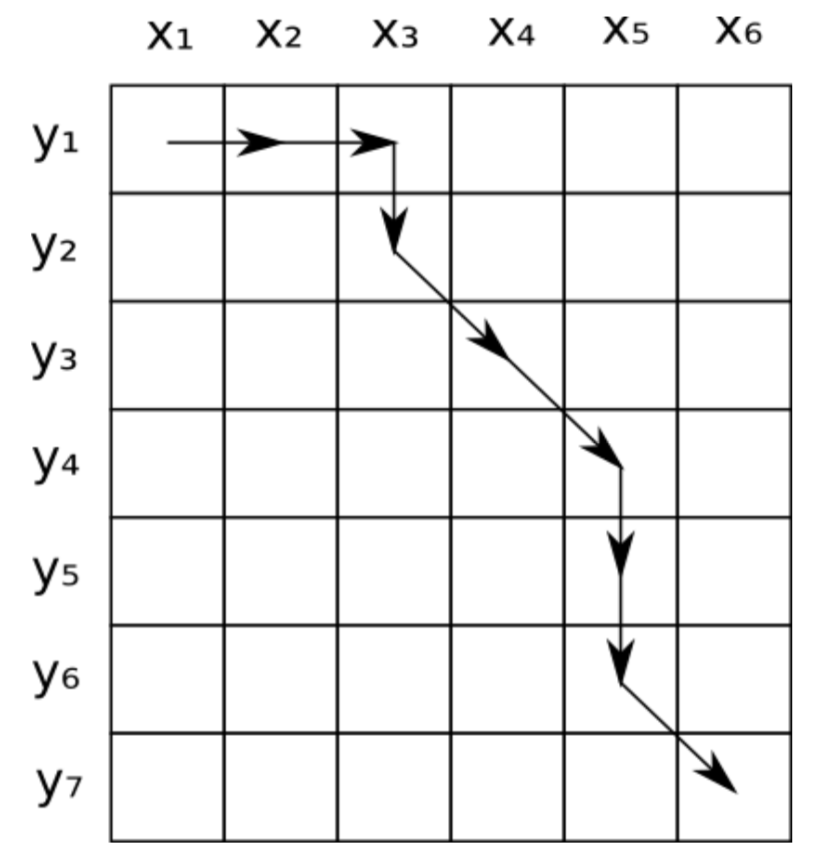
\includegraphics[width=\textwidth]{originals/simple}
         \caption{multi-branch-num-num}
         \label{fig:multi_branch_focussed}
     \end{subfigure}
     \hfill
     \begin{subfigure}[b]{0.3\textwidth}
         \centering
         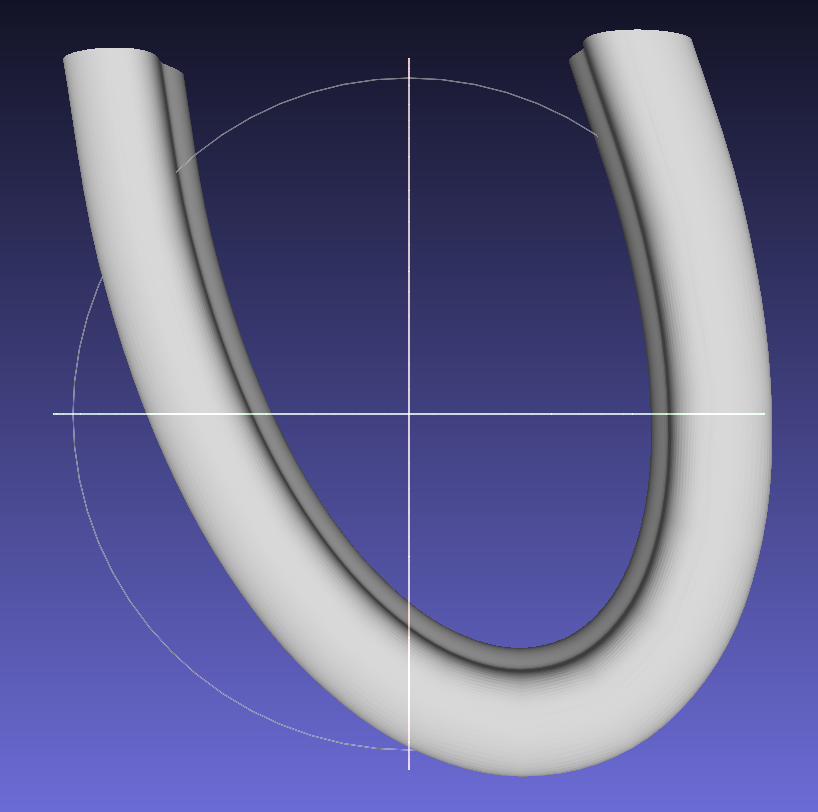
\includegraphics[width=\textwidth]{originals/bend}
         \caption{bend}
         \label{fig:bend}
     \end{subfigure}
        \caption{Original Models}
        \label{fig:original_models}
\end{figure}

\subsection{Measurements}

For reconstruction accuracy, Mackay used the Hausdorff distance filter built into Meshlab, which takes as input a sampled mesh (the mesh to sample points from), and a target mesh (to find the closest distance from each sample point). Many points are sampled and mean distance is reported. Lower mean distance is better. I will refer to the forward direction as when the original synthetic mesh is the sampled mesh, and the reconstructed mesh is the targest mesh, with reverse being the opposite. 

The filter also has parameters related to sampling, such as whether vertices, edges, or faces are sampled. The choices of sample/target meshes and these parameters are important, as the nature of how the models and reconstructions are generated affect different methods differently. For example, all vertices in Mackay's reconstructions are the original points given by plane sampling, and so lie on a face in the original mesh. Hence the reverse Hausdorff distance filter with only vertices sampled gives a measurement of zero. Whereas the proposed method adds additional points, and so is unlikely to achieve this zero measurement. For this reason only faces will be sampled. When it comes to direction, extraneous faces on a target mesh may reduce Hausdorff distance, but extraneous faces on a sampled mesh increase Hausdorff distance (the preferred interpretation). For this reason, in same examined cases a direction may be omitted for reasons which will be explained.

For contour merging and DTW, Mackay's implementation is used. For the proposed method, the same implementation is used except where contour splitting and point angle replace the point correspondence stage. To start with, 50\% angle weight (and 50\% progression) is used in the point angle metric.

\subsubsection{Simple Model Reconstruction}

A simple tube is reconstructed.

\begin{tabular}{ c c }
&
\end{tabular}
\begin{figure}[h]
     \centering
     \begin{minipage}[b]{.38\linewidth}
       \subcaptionbox{Original}
       {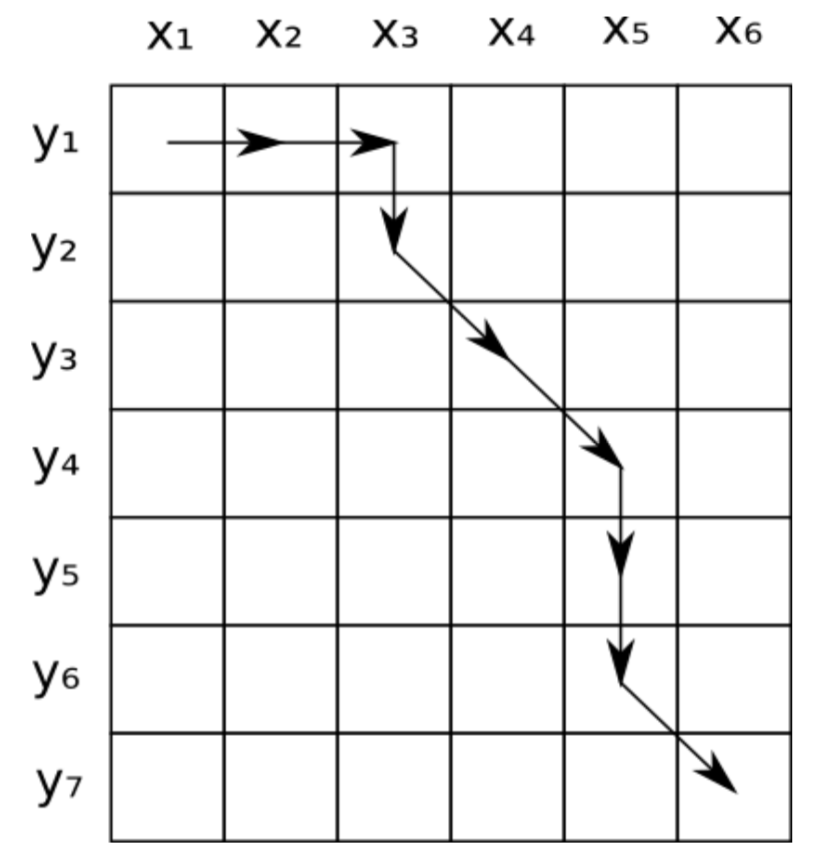
\includegraphics[width=\linewidth]{originals/simple}}%
     \end{minipage}%
     \hfill
     \begin{minipage}[b]{.6\linewidth}
       \subcaptionbox{DTW 50 planes}
       {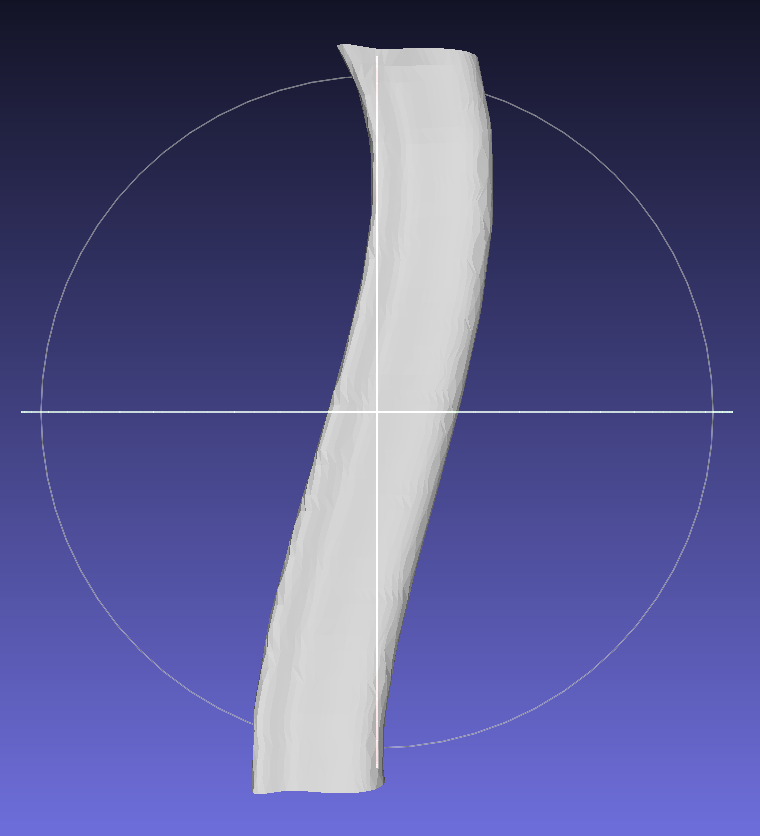
\includegraphics[width=.48\linewidth]{reconstructions/dtw-simple-50}}%
       \hfill
       \subcaptionbox{DTW 10 planes}
       {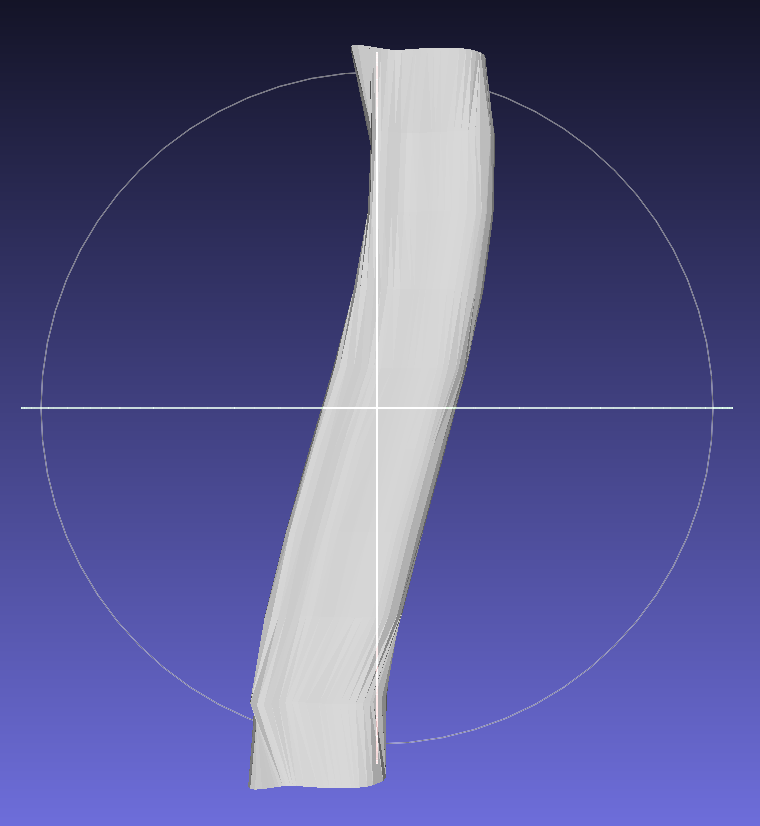
\includegraphics[width=.48\linewidth]{reconstructions/dtw-simple-10}}
       \hfill
       \subcaptionbox{CSPA 50 planes}
       {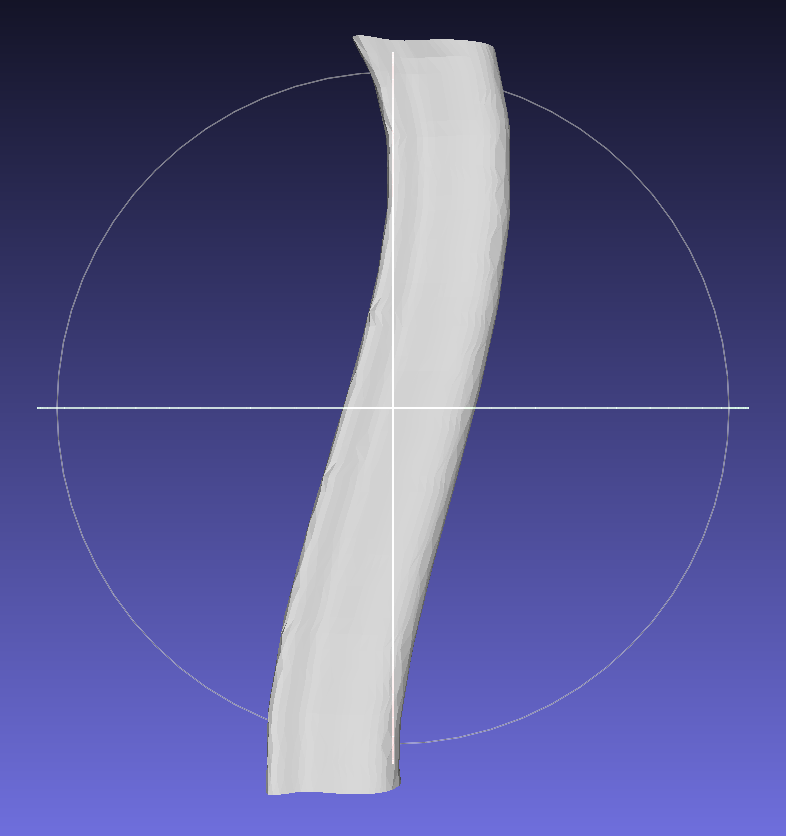
\includegraphics[width=.48\linewidth]{reconstructions/cspa50-simple-50}}%
       \hfill
       \subcaptionbox{CSPA 10 planes}
       {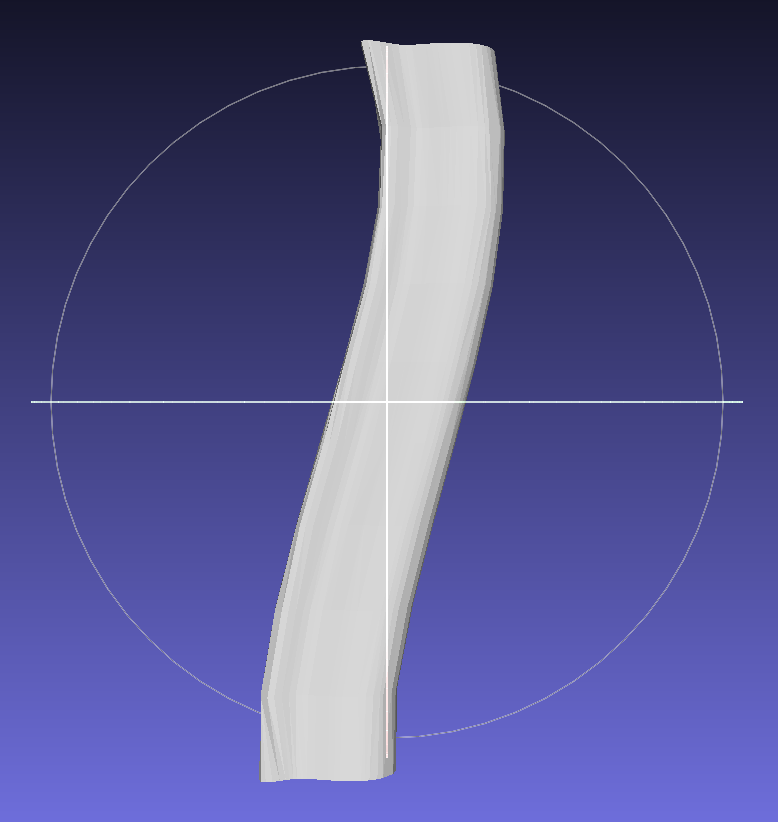
\includegraphics[width=.48\linewidth]{reconstructions/cspa50-simple-10}}
     \end{minipage}%
        \caption{Reconstructions of simple model}
        \label{fig:simple_reconstructions}
\end{figure}

Both reconstruction methods handle this simple case well, with both 50 and 10 plane samples. In the 10 plane reconstruction, they both have visible jagged parts at the bottom, although CSPA seems to be better in this area. We now look at Hausdorff distance to confirm this.

\begin{table}[h]
\begin{tabular}{ | c | c | c | c | c | c | }
\hline
& \multicolumn{5}{c|}{No. of Slices Sampled} \\
\cline{2-6}
Method & 10 & 20 & 30 & 40 & 50 \\
\hline
Contour Merging + DTW (MDTW) & 0.0368 & 0.0274 & 0.0174 & 0.0195 & 0.0145 \\
Contour Splitting + Point Angle (CSPA) & 0.0297 & 0.0240 & 0.0165 & 0.0190 & 0.0140 \\
\hline
\end{tabular}
\caption{Simple model, mean Hausdorff distance from original to reconstruction}
\label{table:simple_forward}
\end{table}

In Table \ref{table:simple_forward}, the anamoly at 40 samples is caused by the 40 plane samples not spanning the full original model. This affects both methods equivalently so has been left in for relative comparison.

\begin{table}[h]
\begin{tabular}{ | c | c | c | c | c | c | }
\hline
& \multicolumn{5}{c|}{No. of Slices Sampled} \\
\cline{2-6}
Method & 10 & 20 & 30 & 40 & 50 \\
\hline
Contour Merging + DTW (MDTW) & 0.0186 & 0.00836 & 0.00479 & 0.00336 & 0.00275 \\
Contour Splitting + Point Angle (CSPA) & 0.0102 & 0.00401 & 0.00281 & 0.00236 & 0.00215 \\
\hline
\end{tabular}
\caption{Simple model, mean Hausdorff distance from reconstruction to original}
\label{table:simple_reverse}
\end{table}

\begin{figure}[h]
\centering
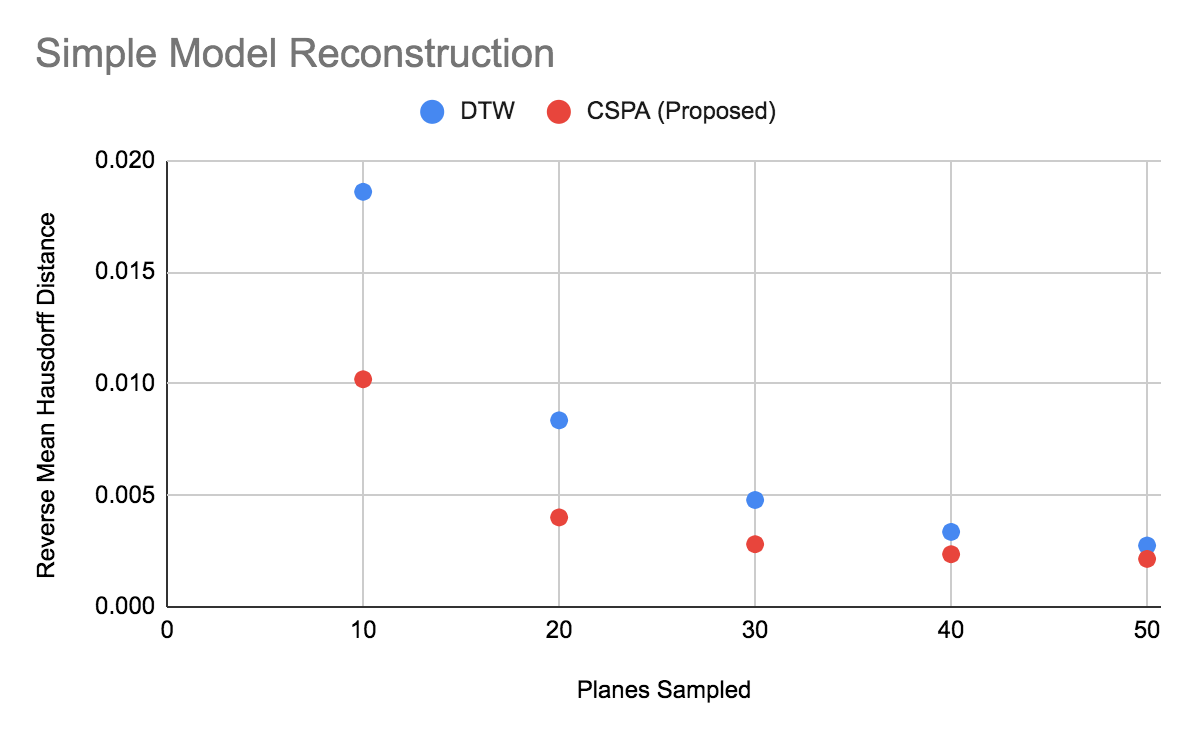
\includegraphics[width=0.9\textwidth]{graphs/simple-reverse}
\caption{Simple model, mean Hausdorff distance from reconstruction to original\label{fig:simple_reverse_graph}}
\end{figure}

As we can see, this agrees with the trend in Mackay's measurements, in that more slices sampled results in more accurate reconstructions. At high sample rates, the two methods have similar accuracies. However, as the sample rate lowers, CSPA has better measured accuracy than MDTW. This is a trend which will continue for the remaining models.

\subsubsection{Simple Branch Reconstruction}

A simple model containing a branch is reconstructed.

(figures)

(figure discussion)

20 and 50 plane samples had invalid contour correspondence.

\begin{table}[h]
\begin{tabular}{ | c | c | c | c | c | c | }
\hline
& \multicolumn{5}{c|}{No. of Slices Sampled} \\
\cline{2-6}
Method & 10 & 20 & 30 & 40 & 50 \\
\hline
Contour Merging + DTW (MDTW) & 0.0727 & - & 0.0641 & 0.0605 & - \\
Contour Splitting + Point Angle (CSPA) & 0.0685 & - & 0.0640 & 0.0607 & - \\
\hline
\end{tabular}
\caption{Simple branch model, mean Hausdorff distance from original to reconstruction}
\label{table:simple_branch_forward}
\end{table}

In between text

\begin{table}[h]
\begin{tabular}{ | c | c | c | c | c | c | }
\hline
& \multicolumn{5}{c|}{No. of Slices Sampled} \\
\cline{2-6}
Method & 10 & 20 & 30 & 40 & 50 \\
\hline
Contour Merging + DTW (MDTW) & 0.0195 & - & 0.0107 & 0.0538 & - \\
Contour Splitting + Point Angle (CSPA) & 0.0147 & - & 0.0115 & 0.0768 & - \\
\hline
\end{tabular}
\caption{Simple branch model, mean Hausdorff distance from reconstruction to original}
\label{table:simple_branch_reverse}
\end{table}

simple discussion (examine 40 sample version)

We follow this up with a model focussing on the branch section of the simple branch model. This entails comparing the complete simple model reconstruction to this focussed original model. Only the forward Hausdorff distance is valid here.

\begin{table}[h]
\begin{tabular}{ | c | c | c | c | c | c | }
\hline
& \multicolumn{5}{c|}{No. of Slices Sampled} \\
\cline{2-6}
Method & 10 & 20 & 30 & 40 & 50 \\
\hline
Contour Merging + DTW (MDTW) & 0.0315 & - & 0.00453 & 0.00440 & - \\
Contour Splitting + Point Angle (CSPA) & 0.0207 & - & 0.00469 & 0.00482 & - \\
\hline
\end{tabular}
\caption{Simple branch focussed model, mean Hausdorff distance from original to reconstruction}
\label{table:simple_branch_focussed_forward}
\end{table}

\subsubsection{Multi Branch Reconstruction}

multi branch

\begin{table}[h]
\begin{tabular}{ | c | c | c | c | c | c | }
\hline
& \multicolumn{5}{c|}{No. of Slices Sampled} \\
\cline{2-6}
Method & 10 & 20 & 30 & 40 & 50 \\
\hline
Contour Merging + DTW (MDTW) & 0.416 & 0.0629 & 0.0264 & 0.0261 & 0.0138 \\
Contour Splitting + Point Angle (CSPA) & 0.404 & 0.0462 & 0.0414 & 0.0255 & 0.0144 \\
\hline
\end{tabular}
\caption{Multi branch model, mean Hausdorff distance from original to reconstruction}
\label{table:multi_branch_forward}
\end{table}

In between text

\begin{table}[h]
\begin{tabular}{ | c | c | c | c | c | c | }
\hline
& \multicolumn{5}{c|}{No. of Slices Sampled} \\
\cline{2-6}
Method & 10 & 20 & 30 & 40 & 50 \\
\hline
Contour Merging + DTW (MDTW) & 0.0964 & 0.0469 & 0.0320 & 0.0400 & 0.0236 \\
Contour Splitting + Point Angle (CSPA) & 0.0773 & 0.0371 & 0.0157 & 0.0350 & 0.0135 \\
\hline
\end{tabular}
\caption{Multi branch model, mean Hausdorff distance from reconstruction to original}
\label{table:multi_branch_reverse}
\end{table}

jwddjnw

\subsubsection{Bend Reconstruction}

In this section a bended tube is reconstructed. This tube is oriented so that when scanned, it appears as two contours coming down to one, similar to a branch.

\begin{table}[h]
\begin{tabular}{ | c | c | c | c | c | c | }
\hline
& \multicolumn{5}{c|}{No. of Slices Sampled} \\
\cline{2-6}
Method & 10 & 20 & 30 & 40 & 50 \\
\hline
Contour Merging + DTW (MDTW) & 0.0764 & 0.0363 & 0.0321 & 0.0314 & 0.0266 \\
Contour Splitting + Point Angle (CSPA) & 0.0647 & 0.0325 & 0.0281 & 0.0296 & 0.0256 \\
\hline
\end{tabular}
\caption{Bend model, mean Hausdorff distance from original to reconstruction}
\label{table:bend_forward}
\end{table}

In between text

\begin{table}[h]
\begin{tabular}{ | c | c | c | c | c | c | }
\hline
& \multicolumn{5}{c|}{No. of Slices Sampled} \\
\cline{2-6}
Method & 10 & 20 & 30 & 40 & 50 \\
\hline
Contour Merging + DTW (MDTW) & 0.0618 & 0.0469 & 0.0158 & 0.101 & 0.0761 \\
Contour Splitting + Point Angle (CSPA) & 0.0535 & 0.0371 & 0.0128 & 0.0650 & 0.0481 \\
\hline
\end{tabular}
\caption{Bend model, mean Hausdorff distance from reconstruction to original}
\label{table:bend_reverse}
\end{table}

a

\subsection{Summary}

summary text

\section{Conclusion}

conclusion text

\pagebreak
\bibliographystyle{IEEEtran}
\bibliography{references}

\section{Appendix}

\begin{figure}[h]
\centering
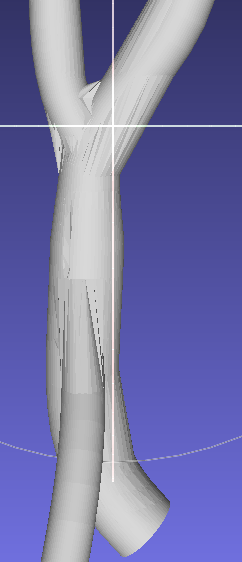
\includegraphics[width=0.29\textwidth]{mb}
\caption{Original multi branch model\label{fig:model}}
\end{figure}

\end{document}
